% =====================================================================
%  WP4 (spatially-honest cross-validation) + WP5 (MAUP / exposure sensitivity)
%  Methods and Results subsections — drop-in fragment, v1
%
%  Owner:   Geospatial Lead
%  Status:  DRAFT for PI review. Not yet assigned to a manuscript.
%  Date:    2026-08-15
%
%  WHY THIS IS A SEPARATE FILE, NOT AN EDIT TO A MANUSCRIPT
%  --------------------------------------------------------
%  Two governance items are unresolved: (1) PR #8's FINAL_CANONICAL_DECISION.md
%  places M6/WP4/WP5 outside Paper 1 evidence pending PI direction, and (2) the
%  Paper 1 vs Paper 2 assignment for the geomatics work has been put to the PI
%  and not answered. These subsections are therefore written to be dropped into
%  whichever manuscript the PI designates, and are held outside the v44 tree
%  until instruction_m6.md §22 is resolved.
%
%  SCOPE OF WHAT IS REPORTED HERE
%  ------------------------------
%  Everything below is computed and executed. Two registered analyses are NOT
%  here because they are blocked on the §5.1 artifacts (the design matrices):
%    * WP5, plan §3.3 registered re-run: dAUC and dcalibration under Builds B
%      and C, which require refitting rather than perturbing frozen predictions.
%    * WP4, cross-model re-run: M0/M1/M2/M5 re-evaluated under the spatial
%      folds. The repo holds predictions, not design matrices.
%  Both are marked \REGBLOCK in the text below. Everything else stands on
%  artifacts held locally and is traceable through
%  wp4_wp5_number_provenance_v1.md.
%
%  DEPENDENCIES
%  ------------
%  * New bibliography entries: wp4_wp5_references_add_v1.bib (merge into the
%    manuscript .bib before compiling).
%  * Figures: Manuscript_Figures/wp5/WP5_F2_exposure_contrast.pdf
%             Manuscript_Figures/wp5/WP5_F7_decision_flip_envelope.pdf
%             Manuscript_Figures/wp4/WP4_F_fold_effect_within_m6.pdf
%  * Assumes the host preamble already loads booktabs, graphicx, natbib.
% =====================================================================

% Marker for text that must be revisited if the §5.1 artifacts arrive.
\providecommand{\REGBLOCK}{\textsuperscript{\dag}}

% =====================================================================
%  METHODS
%  Insert after \subsection{Climate exposures and temporal alignment}
% =====================================================================

\subsection{Exposure construction and the three-build exposure ladder}
\label{sec:methods-wp5}

Areal climate exposure is a construction, not an observation: a gridded weather field must be collapsed onto administrative polygons, and the collapse requires a choice of which cells to admit and what to weight them by. Because that choice is analyst-controlled and unreported in most early-warning studies, it is a candidate explanation for any miscalibration we attribute to the models themselves --- the modifiable areal unit problem in its weighting form~\cite{Openshaw1984,Fotheringham1991}. We therefore built the exposure table three ways and propagated all three through the decision analysis, holding the weather fields, the geometry, the outcome labels, the temporal split and the reference threshold fixed.

The three builds form a nested ladder, each adding exactly one refinement. \textbf{Build A} is the incumbent area-weighted construction: every grid cell touching a polygon is admitted (an \texttt{all\_touched} mask) and cells are averaged with equal weight. \textbf{Build A$'$} replaces that mask with fractional-area weighting, so a cell contributes in proportion to the share of its footprint inside the polygon; isolating this step separates \emph{which cells are admitted} from \emph{what they are weighted by}. \textbf{Build B} re-weights the same admitted cells by the population they contain. \textbf{Build C} additionally corrects temperature for the elevation difference between the reanalysis orography and the population's true elevation before aggregation. Each table carries the same 10{,}842 keys (26 RDHS $\times$ 417 ISO weeks, 2018-01-01 to 2025-12-28) and is row-aligned to the others, so the builds differ from one another by construction alone.

All weighting was performed in an equal-area projection (EPSG:32644); no area or population weight was computed in geographic degrees. Population weights came from WorldPop 100\,m UN-adjusted constrained rasters~\cite{Tatem2017,WorldPop2025}, assigned to (district, climate cell) pairs by pixel centre and normalised within district, so that a district's national population total cancels and only the \emph{shape} of the population surface inside the district can affect exposure. WorldPop UN-adjusted terminates at 2020 against an exposure window ending in 2025, so the plan's vintage-matching requirement could not be met as specified; we instead held the 2020 weight field constant and measured the drift it induces (approximately 1.1\% of a typical weight over 2018--2020), reporting it as a bounded extrapolation rather than imputing later vintages.

Precipitation was taken from CHIRPS v2 daily p05~\cite{Funk2015,CHIRPS} and temperature and dewpoint from ERA5 single-level reanalysis~\cite{Hersbach2020} accessed through the analysis-ready cloud-optimised mirror~\cite{Carver2023ARCO}. Relative humidity was computed per grid cell per hour from temperature and dewpoint by the Alduchov--Eskridge Magnus formulation~\cite{AlduchovEskridge1996} \emph{before} any spatial or temporal averaging; deriving it instead from weekly-mean temperature and dewpoint yields a plausible-looking but incorrect field, because the relation is nonlinear.

\paragraph{Grid resolution, and the direction of its bias.} The pre-specified temperature source was ERA5-Land at $0.1^{\circ}$, which requires a Copernicus Climate Data Store account that was not available to the geospatial analysis environment. Temperature and humidity were therefore built on ERA5 at $0.25^{\circ}$. This substitution attenuates the very effect WP5 measures, and the attenuation was quantified before any exposure table was built, from the digital elevation model and the population raster alone: at $0.25^{\circ}$ the population-weighted construction recovers 65.3\% of the elevation displacement it would recover at $0.1^{\circ}$ (91.7\%), and the effective number of contributing cells per district falls from 21.3 (area) and 11.8 (population) to 5.3 and 3.6. The bias therefore runs \emph{toward the null}, so every temperature displacement reported below is a conservative floor. The same attenuation makes district-level attributions unreliable for the A$'\to$B temperature step in the most strongly attenuated districts (Ratnapura retains 6.7\% of its predicted shift), and we make no claim about \emph{which} districts warm under population weighting on that rung. Precipitation is unaffected: CHIRPS was used at its native $0.05^{\circ}$ in every build.

\paragraph{Build C: correcting to the elevation the reanalysis believes.} A lapse-rate correction requires two elevations, not one --- the true population-weighted elevation and the elevation the reanalysis implicitly assumes. We took the latter from ERA5's own surface geopotential, which is distributed in the same store as the temperature fields and was verified invariant across hours and across years. Correcting to a digital elevation model without it --- the natural shortcut --- assumes the reanalysis already sits at true mean elevation, which is precisely what fails in the highlands: ERA5's orography over Sri Lanka peaks at 1{,}219\,m against the island's true 2{,}524\,m. Temperature and dewpoint were corrected at the environmental lapse rate ($6.5\,^{\circ}$C\,km$^{-1}$; $1.5\,^{\circ}$C\,km$^{-1}$ for dewpoint) with a saturation guard preventing dewpoint from exceeding temperature, then aggregated under the Build B population weights, so the B$\to$C step isolates terrain on top of population weighting. Because the correction is affine in elevation, correcting each fine-grid pixel and then aggregating is exactly equivalent to correcting the weighted-mean elevation, which we verified; relative humidity is the exception and was recomputed per cell per hour from the corrected fields rather than patched onto the aggregate. Copernicus GLO-30 supplied the terrain~\cite{CopernicusDEM2021}. Precipitation carries no Build C rung: CHIRPS is an observational product calibrated to gauges, not a reanalysis with an internal orography to correct against, and constructing an orographic-enhancement model would violate the study's no-new-model rule.

\paragraph{Independent validation of Build C.} Because Build C is the one rung that asserts a physical correction rather than a re-weighting, it was validated against station observations rather than accepted on construction. GHCN-Daily~\cite{Menne2012} provides six Sri Lankan stations reporting through 2025, one of them at Nuwara Eliya at 1{,}880\,m and the remainder between 1.8 and 116\,m. Station daily means were compared with ERA5 daily means on local (UTC+5:30) days.

\paragraph{Population-product sensitivity.} Because Build B rests on a single modelled population surface, the weight field was rebuilt under two alternatives at the same 2020 epoch: WorldPop R2025A constrained (a newer release from the same producer) and GHS-POP R2023A~\cite{Schiavina2023}, which is produced by a different institution using a built-up-surface dasymetric method rather than a random forest. The fourth arm named in the analysis plan --- census district totals --- is degenerate and was struck rather than run: totals carry no within-district spatial information, so distributing them uniformly reproduces Build A exactly, and the totals themselves cancel in the within-district normalisation.

\paragraph{Decision sensitivity.} The registered form of this analysis refits the model ladder under each build and reports $\Delta$AUC, $\Delta$calibration and $\Delta$NB; it requires the model design matrices, which the frozen analysis archive does not contain (it holds predictions), and it is not reported here\,\REGBLOCK. The question \emph{does the alert decision move?} does not require refitting, and we answer it within a bounded envelope constructed from three pieces. First, an exact model-free \emph{flip curve}: a held-out row can change its alert status only if its predicted risk lies within the applied perturbation of the threshold, so $\#\{|p-p^*|\le\delta\}$ bounds the flips attributable to \emph{any} perturbation of size $\delta$, whatever generates it. Second, an observed \emph{ceiling}: the alert changes produced by deleting the entire climate block, computed on identical rows from the frozen full and climate-free predictions. Third, a \emph{transfer coefficient} $\beta$ relating exposure to predicted risk, estimated by regressing $\mathrm{logit}(p_{\mathrm{full}})-\mathrm{logit}(p_{\mathrm{noclim}})$ on the exposure variables --- which needs the predictions only. We estimated $\beta$ under four specifications (exposure alone; plus district fixed effects; plus seasonal harmonics; plus both) and report the range across all four rather than a single fit, because the specification is not identified without the design matrices. Every estimated flip count is asserted against the exact flip curve in the analysis notebook. Uncertainty used the study's established protocol: percentile intervals from 2{,}000 cluster-bootstrap resamples of the 26 RDHS units, seed 20260612~\cite{CameronGelbachMiller2008}.

\subsection{Spatially-honest cross-validation}
\label{sec:methods-wp4}

The study's held-out evaluation is a single temporal split, which leaves the external-validation claim exposed to a spatial objection: neighbouring units share weather and outbreak timing, so a model trained on a district's neighbours has seen much of that district's signal. WP4 addresses this with buffered leave-one-out cross-validation, sized to Sri Lanka's 26 units~\cite{Roberts2017,Valavi2019}.

\paragraph{Fold construction and the leakage audit.} For each of the 26 RDHS units in turn, the unit was held out and the training set additionally excluded every unit within a buffer radius of it. Distance was measured \emph{boundary-to-boundary} in the equal-area projection, not centroid-to-centroid: adjacent Sri Lankan districts sit 28--119\,km apart by centroid while sharing a border, so a centroid buffer would apply a wildly uneven exclusion. Folds were built as a function of radius (0, 10, 25, 50, 75, 100 and 150\,km, plus graph-hop variants) so that the operative radius could be selected from the autocorrelation analysis without rebuilding. Hop-based and kilometre-based buffers are not interchangeable --- one graph hop removes between 2 and 7 districts depending on location, applying an uneven buffer while appearing uniform --- and the kilometre buffers are treated as primary. The spatial half of the leakage audit was asserted rather than assumed: for every radius and every fold, zero train--test unit pairs fall within the buffer. Temporal honesty is enforced upstream, where a composite predictor is admissible for week $W$ only if its averaging window \emph{ended} before $W$ began; the two constraints are orthogonal, so the scheme is spatio-temporal.

\paragraph{Residual autocorrelation range.} The buffer radius was to be set from the residual spatial autocorrelation range. Moran's $I$ was computed per test week across distance bands on the adjacency graph and tested against a permutation null (999 shuffles, seed 20260612), and an empirical variogram was fitted over 0--400\,km, for the frozen full and climate-free models and for the geomatics-only model.

\paragraph{Measuring what the folds cost.} Re-evaluating the published model ladder under these folds requires refitting each model, hence each model's design matrix, which the frozen archive does not contain\,\REGBLOCK; a spatially cross-validated model set against a temporally split comparator would be an artifact of the schemes rather than a comparison. We therefore measured the fold effect as a \emph{within-model} contrast, on the geomatics-only model, where features and labels are held locally: the same model, the same features, the same 3{,}926 held-out rows, with only the validation scheme changing. This is a stricter instrument than the cross-model version, because nothing else varies.

The design point is the control. Buffering a fold removes spatial leakage \emph{and} training data, and both depress performance, so a raw buffered-versus-temporal comparison measures sample size and calls it leakage. Every buffered fold was therefore matched against a \emph{random-district control} trained on an identical number of districts, drawn without regard to geography (10 draws per radius); the buffered-minus-matched-control gap is the part attributable to geography, and the remainder is the price of a smaller training set. Across four arms this required 1{,}456 model fits. Two gates were passed before any contrast was read: the rebuilt outcome labels reproduce the frozen outcomes on all 3{,}926 test rows, and the baseline arm reproduces the committed model's predictions to $8.6\times10^{-15}$. Uncertainty used the same cluster bootstrap as above (2{,}000 replicates, districts resampled, seed 20260612), with the control ensemble averaged inside each replicate.

Per the analysis plan's power caveat, the Sri Lanka spatial result is a compact-country sensitivity companion; the well-powered spatial claim rests on the Colombia block cross-validation over approximately 1{,}000 municipalities, which is outside the scope of the Sri Lanka analysis reported here.

% =====================================================================
%  RESULTS
%  Insert after \subsection{Threshold and stricter-outcome robustness}
% =====================================================================

\subsection{Exposure construction moves exposure}
\label{sec:results-wp5-exposure}

Exposure construction moved every variable measured, so the pre-specified honest-null clause fired on none of them (Table~\ref{tab:wp5-ladder}, Fig~\ref{fig:wp5f2}). Across 10{,}842 district-weeks, replacing area weighting with population weighting displaced weekly rainfall by a mean absolute 3.40\,mm (7.9\% of the 42.9\,mm mean weekly rainfall), with a largest single district-week of 72.6\,mm; weekly mean temperature by 0.205\,$^{\circ}$C; weekly maximum temperature by 0.387\,$^{\circ}$C; and relative humidity by 0.77 percentage points. The lapse correction moved weekly mean temperature by a further 0.306\,$^{\circ}$C.

Four features of that displacement matter more than its magnitude.

\emph{The mask is a footnote; the weights are the result.} Decomposing A$\to$B into its two steps, exchanging the \texttt{all\_touched} mask for fractional-area weighting moved 1.8\% of mean rainfall, while re-weighting from area to population moved 7.9\%. What an exposure table is weighted by matters roughly four times more than which cells it admits --- and it is the weighting, not the mask, that studies leave unreported.

\emph{The rungs act on different parts of the distribution.} Population weighting moved the weekly \emph{maximum} temperature roughly twice as far as the weekly mean (0.387 against 0.205\,$^{\circ}$C, with a maximum of 2.76\,$^{\circ}$C), because it re-weights a field whose cells disagree most in the tails. For a transmission process governed by thermal limits rather than averages, the tail is the relevant quantity. The lapse correction, being one offset per district, moved minimum, mean and maximum identically.

\emph{In the weeks that would trigger an alert, the rainfall contrast grows in millimetres and shrinks in percent.} In the wettest decile of district-weeks the displacement was 8.6\,mm (5.4\%) and in the wettest percentile 12.9\,mm (4.9\%). A decision analysis feels the millimetres; a bias argument feels the percentage. Relatedly, the correlation between the two arms (0.9935 for rainfall) is not the reassurance it appears to be, because the table is dominated by dry weeks.

\emph{Exposure sensitivity is not a property of a district.} Ranked by absolute displacement, rainfall and temperature share only one district in their top five, and the rank correlation between them is indistinguishable from zero ($\rho=0.24$, $p=0.23$). A single-variable sensitivity check will therefore identify the wrong set of exposure-sensitive districts, and no single such map exists. The signs are nonetheless geographic rather than noisy: Colombo loses 7.30\,mm per week of rainfall under population weighting and Puttalam gains 4.37, as people cluster on the drier coastal strip in the first case and away from it in the second; 17 districts move down and 9 up.

\paragraph{The lapse correction, and what part of it belongs to MAUP.} On the grid available the lapse correction moved exposure about 1.5 times as far as population weighting did (0.306 against 0.205\,$^{\circ}$C), reversing the ranking anticipated in the analysis plan. That reversal is a resolution effect and it is coherent: what the correction recovers is exactly what a coarse grid loses, so it grows as the grid coarsens, and it is the one rung that partly repairs the missing $0.1^{\circ}$ product rather than being degraded by it. The largest district shifts were Nuwara Eliya $-1.92\,^{\circ}$C, Badulla $-1.33\,^{\circ}$C and Ratnapura $+1.01\,^{\circ}$C.

The B$\to$C step must not be reported as a MAUP effect in full. Decomposed, a mean 0.223\,$^{\circ}$C is an orography deficit --- ERA5 issuing temperature for a mountain range about half its true height --- which would apply under area weighting too and belongs to the exposure-\emph{quality} argument, while 0.169\,$^{\circ}$C is genuine sub-grid population placement and is the only part belonging to WP5's exposure-\emph{construction} argument. The two can oppose each other (in Nuwara Eliya, $-2.26$ and $+0.34\,^{\circ}$C), so quoting the combined figure as MAUP would overstate the result by roughly half.

\paragraph{Station validation.} ERA5 is accurate at sea level over Sri Lanka and approximately 5\,$^{\circ}$C too warm in the highlands --- an elevation-dependent bias, which is what Build C models, not a global offset. Against GHCN-Daily, the Nuwara Eliya station (1{,}880\,m) records 16.40\,$^{\circ}$C against ERA5's 21.17\,$^{\circ}$C (bias $+4.77\,^{\circ}$C), while four well-sampled lowland stations (1.8--116\,m) sit between $-0.36$ and $-0.42\,^{\circ}$C; the pattern holds in every year 2018--2025 and in both daily maxima and minima. Regressing the five well-sampled stations on elevation gives a local lapse rate of $6.40\,^{\circ}$C\,km$^{-1}$, and ERA5's own between-cell lapse over land is $6.31\,^{\circ}$C\,km$^{-1}$, both within about 2\% of the $6.5\,^{\circ}$C\,km$^{-1}$ applied, so no rescaling is warranted. Interpolating the station regression to Nuwara Eliya's population-weighted elevation (1{,}260\,m) implies a true district mean of 19.82\,$^{\circ}$C, against Build B's 21.89 (error $+2.07$) and Build C's 19.98 (error $+0.15$): the correction removes 93\% of the error where it is largest. Three limits bound this: the high end of the regression rests on a single station; the larger bias in daily minima ($+5.27$) than maxima ($+4.27$) is the signature of nocturnal cold-air pooling in a highland basin, a local siting effect that should not be extrapolated to a district's whole population; and the correction remains anchored to ERA5's smoothed orography, so a $0.1^{\circ}$ rebuild would start from a better one.

\subsection{Exposure construction changes alert decisions, and net benefit cannot see it}
\label{sec:results-wp5-decision}

At the reference threshold $p^*=0.30$, exposure construction changed the alert decision on 35--76 held-out district-weeks (0.9--1.9\%) for the A$'\to$B step and 64--104 (1.6--2.6\%) for A$'\to$C, the range spanning the four transfer specifications (Table~\ref{tab:wp5-flips}, Fig~\ref{fig:wp5f7}). For scale, deleting the entire climate block from the model changed 441 decisions (11.2\%) on the same rows. Exposure construction alone therefore carries 14--24\% of the climate block's entire decision leverage --- far from nothing, and far from everything. Under the district-fixed-effects specification, cluster-bootstrap intervals were 1.94\% [1.27, 2.65] for A$'\to$B and 2.45\% [1.50, 3.57] for A$'\to$C, against 11.23\% [9.40, 13.17] for climate removal. In operational terms, at 26 districts and 52 weeks a 1.9\% flip rate is approximately 26 changed alert decisions per year nationally, against approximately 152 for the presence or absence of climate information altogether.

These estimates are bounded from above by a quantity that requires no model at all. Because a row can change its alert status only if its predicted risk lies within the applied perturbation of the threshold, and only 6.4\% of held-out rows lie within 0.02 of $p^*=0.30$ on the recalibrated scale (6.0\% on the raw scale), no perturbation of that size can flip more than 6.4\% of decisions however it is generated. Every estimate above is asserted against that exact bound. The transfer coefficient's norm varies by a factor of 2.3 across the four specifications ($R^2$ 0.27--0.38, signs stable throughout), but the flip count varies far less, because the flip curve is locally near-linear --- the coefficient would have to be understated several-fold before exposure construction approached the ceiling. The qualitative answer is therefore robust to what the blocked refit would supply.

\paragraph{A near-zero $\Delta$NB is not evidence of decision insensitivity.} Across every rung, specification and threshold examined, the change in net benefit remained within $\pm0.0023$ while the flip counts above were unambiguously non-zero. This is not flips cancelling by direction: they are strongly asymmetric (A$'\to$B at $p^*=0.30$ added 67 alerts and removed 9). It is structural, and it follows from the definition of the decision-analytic threshold. A row can flip only if it sits near $p^*$; rows near $p^*$ have an event rate near $p^*$; and $p^*$ is by construction the break-even rate at which a true positive and the corresponding false positives are worth the same. Every flip is therefore worth approximately zero net benefit in either direction. Measured, the event rate among flipped rows tracks $p^*$ across both rungs and all four thresholds (0.087, 0.160, 0.289 and 0.431 against thresholds of 0.10, 0.20, 0.30 and 0.40; $r=0.96$), and the arithmetic closes exactly.

The implication is general and reaches beyond this study: \emph{net benefit is structurally insensitive to any perturbation acting near the decision threshold}, so a near-zero $\Delta$NB must not be reported as evidence that a perturbation does not affect decisions. It answers a different question --- whether the perturbation changes the value of the alerts --- from the one a decision-flip count answers. Any sensitivity analysis in this literature that concludes ``no decision effect'' from a small $\Delta$NB alone is subject to this critique, including several reported elsewhere in this paper; we accordingly report flip counts alongside $\Delta$NB throughout.

Finally, flips require a displacement \emph{and} a prediction near the threshold. Across the 26 districts the flip count correlates with the induced prediction shift but not with exposure displacement alone --- so, one step beyond the finding above, naming ``exposure-sensitive districts'' from an exposure contrast names the wrong set for decisions as well.

\subsection{The exposure result is not an artifact of the population product}
\label{sec:results-wp5-product}

The most direct objection to a population-weighted exposure result is that it inherits the errors of a single modelled population surface. It does not (Table~\ref{tab:wp5-product}). Rebuilding the weight field under WorldPop R2025A and GHS-POP R2023A moved 2.0\% and 1.6\% of a district's weight respectively, against 27.5\% for the area-to-population step itself. On exposure the separation is an order of magnitude or more: the product swap moved weekly mean temperature by 0.006--0.009\,$^{\circ}$C against 0.205 for the construction step, and rainfall by 0.16--0.20\,mm against 3.40. Ratios of construction effect to product effect run from 16.7 to 32.1 across variables; they do not narrow in the tails where alerts fire (19.5 in the wettest percentile of district-weeks, 35.8 in the hottest); and in 0 of 26 districts does the product effect reach the weighting effect. The per-district reading survives as well, with rank correlations of 0.985 and 0.990 on the ranking of movers, identical top-five sets and complete sign agreement, so the statements above about which districts are exposure-sensitive are not statements about WorldPop.

Two incidental findings are worth recording. First, version drift within one producer exceeded the gap between producers: WorldPop UN-adjusted and WorldPop's own R2025A differ more (mean total variation 0.0201) than WorldPop and GHS-POP do (0.0157), so ``same producer, newer release'' is not the safer substitution it appears to be. Second, the approximately 1.4\% of population that falls outside the 26 polygons under WorldPop UN-adjusted is a coastline artifact specific to that product and vintage: on identical boundaries GHS-POP loses 0.23\% and WorldPop R2025A 0.10\%. It should be reported as a bounded product sensitivity rather than treated as a property of the geometry.

These three products are all modelled surfaces sharing much of their input census, so their agreement bounds method sensitivity, not the truth of where people live. And this analysis addresses exposure only; whether the product choice moves net benefit belongs to the blocked refit\,\REGBLOCK.

\subsection{Spatial cross-validation}
\label{sec:results-wp4}

\paragraph{The power cost, quantified.} Sri Lanka is approximately 430\,km end to end, so a buffer is necessarily a large fraction of the country (Table~\ref{tab:wp4-power}). Excluding only immediately adjacent districts leaves a median of 21 of 25 possible training districts (worst fold 16) and retains 84\% of training district-weeks. At 100\,km the median fold trains on 9 districts and the worst on 5, retaining 36\%; at 150\,km the scheme collapses, with 12 of 26 folds keeping fewer than 5 training districts. The plan's qualitative caveat that leave-one-out remains low-powered at $n=26$ is thereby quantified rather than asserted. Across every radius and fold, zero train--test pairs fell within the buffer.

\paragraph{Residual autocorrelation is undetectable, and does not settle the question.} Moran's $I$ on model residuals was indistinguishable from its permutation null at every distance band for all three models examined (permutation $p$ from 0.53 to 0.99), and the empirical variogram was flat from 25 to 400\,km. This is more robust than it first appears: the full model carries district fixed effects, which absorb time-invariant spatial structure and could manufacture a null, but the geomatics-only model carries no fixed effects at all and returns the same answer ($I=0.001$ among adjacent districts, $p=0.99$). With 26 units the permutation null has a standard deviation of approximately 0.02, so this excludes residual spatial correlation above roughly $|I|=0.04$ rather than proving its absence.

\paragraph{The folds are nonetheless expensive.} Direct measurement contradicts the inference that would follow from the residual analysis (Table~\ref{tab:wp4-fold}, Fig~\ref{fig:wp4f}). Against a temporal-split AUC of 0.601 and an unbuffered leave-one-out AUC of 0.592, adjacency buffering scored 0.565 while a random-district control trained on the same 21 districts scored 0.587 --- a geography-attributable gap of $-0.022$. The gap widens with radius, and at 100\,km the spatially blocked estimate is 0.502, indistinguishable from chance, while an equally sized random training set still reaches 0.573. Because training-set size is held fixed by construction, that difference cannot be sample size. In 0 of 10 control draws at 0, 75 and 100\,km did a random subset score below the buffered fold. Calibration degrades along the same gradient, the calibration slope falling from 0.875 under the temporal split to 0.529 at adjacency buffering and 0.018 at 100\,km. The effect is not one district's doing: 17 of 26 districts lose discrimination under adjacency buffering and 9 gain.

Power is the binding constraint on certifying this. Cluster-bootstrap intervals for the buffered-minus-control gap span zero at 0\,km ($-0.022$ [$-0.055$, $+0.011$]) and exclude zero only at 75\,km ($-0.061$ [$-0.119$, $-0.008$]) and 100\,km ($-0.068$ [$-0.143$, $-0.001$]). The point estimates are consistent and one-signed at every radius, but with 26 clusters the bootstrap has little to work with --- the power table above arriving from the other direction. Intervals spanning zero here mean no difference was detected, not that none exists.

The methodological point generalises beyond this model. \emph{Residual spatial autocorrelation and dependence on spatially proximate training data are different quantities, and they can disagree.} Moran's $I$ on residuals asks whether what remains after fitting on every unit is spatially clustered; a buffered fold asks whether a model can generalise to a region it has never seen. A model can pass the first and fail the second, and the model examined here does. Selecting a buffer radius from a residual-range analysis --- the conventional design, and the one this study's own plan specified --- therefore cannot be relied on to price the folds; the price has to be measured directly.

Two limits bound what this establishes. It says nothing about the study's headline model comparison, which cannot be re-fitted under the folds without the design matrices\,\REGBLOCK; if the published hybrid depends on spatial proximity in the way the geomatics-only model does, spatial cross-validation would move it too, which is precisely the reviewer concern this work package exists to answer. And it says nothing about absolute performance: the geomatics-only model's outcome labels are a reconstruction carrying an exploratory-target caveat on 19.2\% of test rows, identical across arms so that it cannot manufacture a between-arm difference, but sufficient to bar quoting any single AUC here as that model's performance.

% =====================================================================
%  TABLES
% =====================================================================

\begin{table}[htbp]
\centering
\caption{\textbf{The exposure ladder: how far each construction step moves exposure.} Mean absolute displacement over 10{,}842 district-weeks (26 RDHS $\times$ 417 ISO weeks, 2018--2025). A$\to$A$'$ exchanges an \texttt{all\_touched} mask for fractional-area weighting; A$'\to$B re-weights area to population; B$\to$C corrects temperature to the population's elevation. Temperature figures are conservative floors (see Methods, grid resolution).}
\label{tab:wp5-ladder}
\begin{tabular}{llrrr}
\toprule
Variable & Step & Mean $|\Delta|$ & Max $|\Delta|$ & \% of mean \\
\midrule
Weekly rainfall (mm)      & A $\to$ A$'$ (mask)   & 0.76  & ---   & 1.8\% \\
Weekly rainfall (mm)      & A$'\to$ B (weights)   & 3.40  & 72.6  & 7.9\% \\
\quad wettest decile      & A$'\to$ B             & 8.56  & ---   & 5.4\% \\
\quad wettest percentile  & A$'\to$ B             & 12.89 & ---   & 4.9\% \\
Weekly mean $T$ ($^{\circ}$C)    & A$'\to$ B      & 0.205 & 1.16  & --- \\
Weekly max $T$ ($^{\circ}$C)     & A$'\to$ B      & 0.387 & 2.76  & --- \\
Weekly min $T$ ($^{\circ}$C)     & A$'\to$ B      & 0.316 & 2.34  & --- \\
Relative humidity (pp)           & A$'\to$ B      & 0.77  & 6.29  & --- \\
Weekly mean $T$ ($^{\circ}$C)    & B $\to$ C      & 0.306 & 1.92  & --- \\
\quad orography component        & B $\to$ C      & 0.223 & ---   & --- \\
\quad sub-grid population component & B $\to$ C   & 0.169 & ---   & --- \\
\bottomrule
\end{tabular}
\end{table}

\begin{table}[htbp]
\centering
\caption{\textbf{Alert decisions changed by exposure construction, $p^*=0.30$.} Held-out panel of 3{,}926 district-weeks (26 RDHS $\times$ 151 weeks, 2023--2025). Ranges span four transfer specifications; intervals are 95\% percentile cluster bootstrap (2{,}000 replicates, districts resampled) under the district-fixed-effects specification. $\Delta$NB is the change in net benefit at the same threshold.}
\label{tab:wp5-flips}
\begin{tabular}{lrrrr}
\toprule
Contrast & Flips & \% of rows & Bootstrap 95\% CI & $|\Delta \mathrm{NB}|$ \\
\midrule
A$'\to$ B (population weighting) & 35--76  & 0.9--1.9  & 1.94 [1.27, 2.65]    & $\le 0.0013$ \\
A$'\to$ C (adds lapse correction) & 64--104 & 1.6--2.6  & 2.45 [1.50, 3.57]    & $\le 0.0009$ \\
Climate block removed (ceiling)   & 441     & 11.2      & 11.23 [9.40, 13.17]  & --- \\
Exact bound, $|p-p^*|\le0.02$     & $\le$253 & $\le$6.4 & ---                  & --- \\
\bottomrule
\end{tabular}
\end{table}

\begin{table}[htbp]
\centering
\caption{\textbf{Population-product sensitivity against the construction effect.} Mean absolute displacement over 10{,}842 district-weeks; weight displacement is mean total variation of the within-district weight vector on the ERA5 grid.}
\label{tab:wp5-product}
\begin{tabular}{lrrrr}
\toprule
Quantity & A$'\to$ B & $\to$R2025A & $\to$GHS-POP & Min.\ ratio \\
\midrule
Weight displaced (\% of district) & 27.5  & 2.0    & 1.6    & 13.8$\times$ \\
Weekly mean $T$ ($^{\circ}$C)     & 0.205 & 0.0088 & 0.0064 & 23.2$\times$ \\
Weekly max $T$ ($^{\circ}$C)      & 0.387 & 0.0231 & 0.0187 & 16.8$\times$ \\
Relative humidity (pp)            & 0.769 & 0.0416 & 0.0319 & 18.5$\times$ \\
Weekly rainfall (mm)              & 3.399 & 0.2032 & 0.1612 & 16.7$\times$ \\
\bottomrule
\end{tabular}
\end{table}

\begin{table}[htbp]
\centering
\caption{\textbf{Power cost of buffered leave-one-out cross-validation, 26 RDHS units.} Training districts available out of 25; distance is boundary-to-boundary in EPSG:32644. A degenerate fold retains fewer than 5 training districts.}
\label{tab:wp4-power}
\begin{tabular}{lrrrr}
\toprule
Buffer & Median train units & Worst fold & Median train district-weeks & Degenerate folds \\
\midrule
Adjacency (0\,km) & 21 & 16 & 5{,}481 & 0 \\
25\,km            & 19 & 14 & 4{,}959 & 0 \\
50\,km            & 15 & 10 & 4{,}045 & 0 \\
75\,km            & 12 & 6  & 3{,}132 & 0 \\
100\,km           & 9  & 5  & 2{,}349 & 0 \\
150\,km           & 5  & 0  & 1{,}435 & 12 \\
\bottomrule
\end{tabular}
\end{table}

\begin{table}[htbp]
\centering
\caption{\textbf{The cost of spatial folds, measured within one model against a size-matched control.} Every buffered fold is matched to a random-district control trained on the same number of districts (10 draws), so the gap isolates geography from sample size. Reference points: temporal split AUC 0.601, unbuffered leave-one-out 0.592. Intervals are 95\% percentile cluster bootstrap (2{,}000 replicates).}
\label{tab:wp4-fold}
\begin{tabular}{lrrrrr}
\toprule
Buffer & Train units & Buffered AUC & Matched control & Gap [95\% CI] & Controls below \\
\midrule
0\,km   & 21 & 0.565 & 0.587 & $-0.022$ [$-0.055$, $+0.011$] & 0 of 10 \\
25\,km  & 19 & 0.571 & 0.590 & $-0.018$ [$-0.058$, $+0.021$] & 1 of 10 \\
50\,km  & 15 & 0.558 & 0.577 & $-0.018$ [$-0.054$, $+0.018$] & 2 of 10 \\
75\,km  & 12 & 0.516 & 0.578 & $-0.061$ [$-0.119$, $-0.008$] & 0 of 10 \\
100\,km & 9  & 0.502 & 0.573 & $-0.068$ [$-0.143$, $-0.001$] & 0 of 10 \\
\bottomrule
\end{tabular}
\end{table}

% =====================================================================
%  FIGURES
% =====================================================================

\begin{figure}[htbp]
\centering
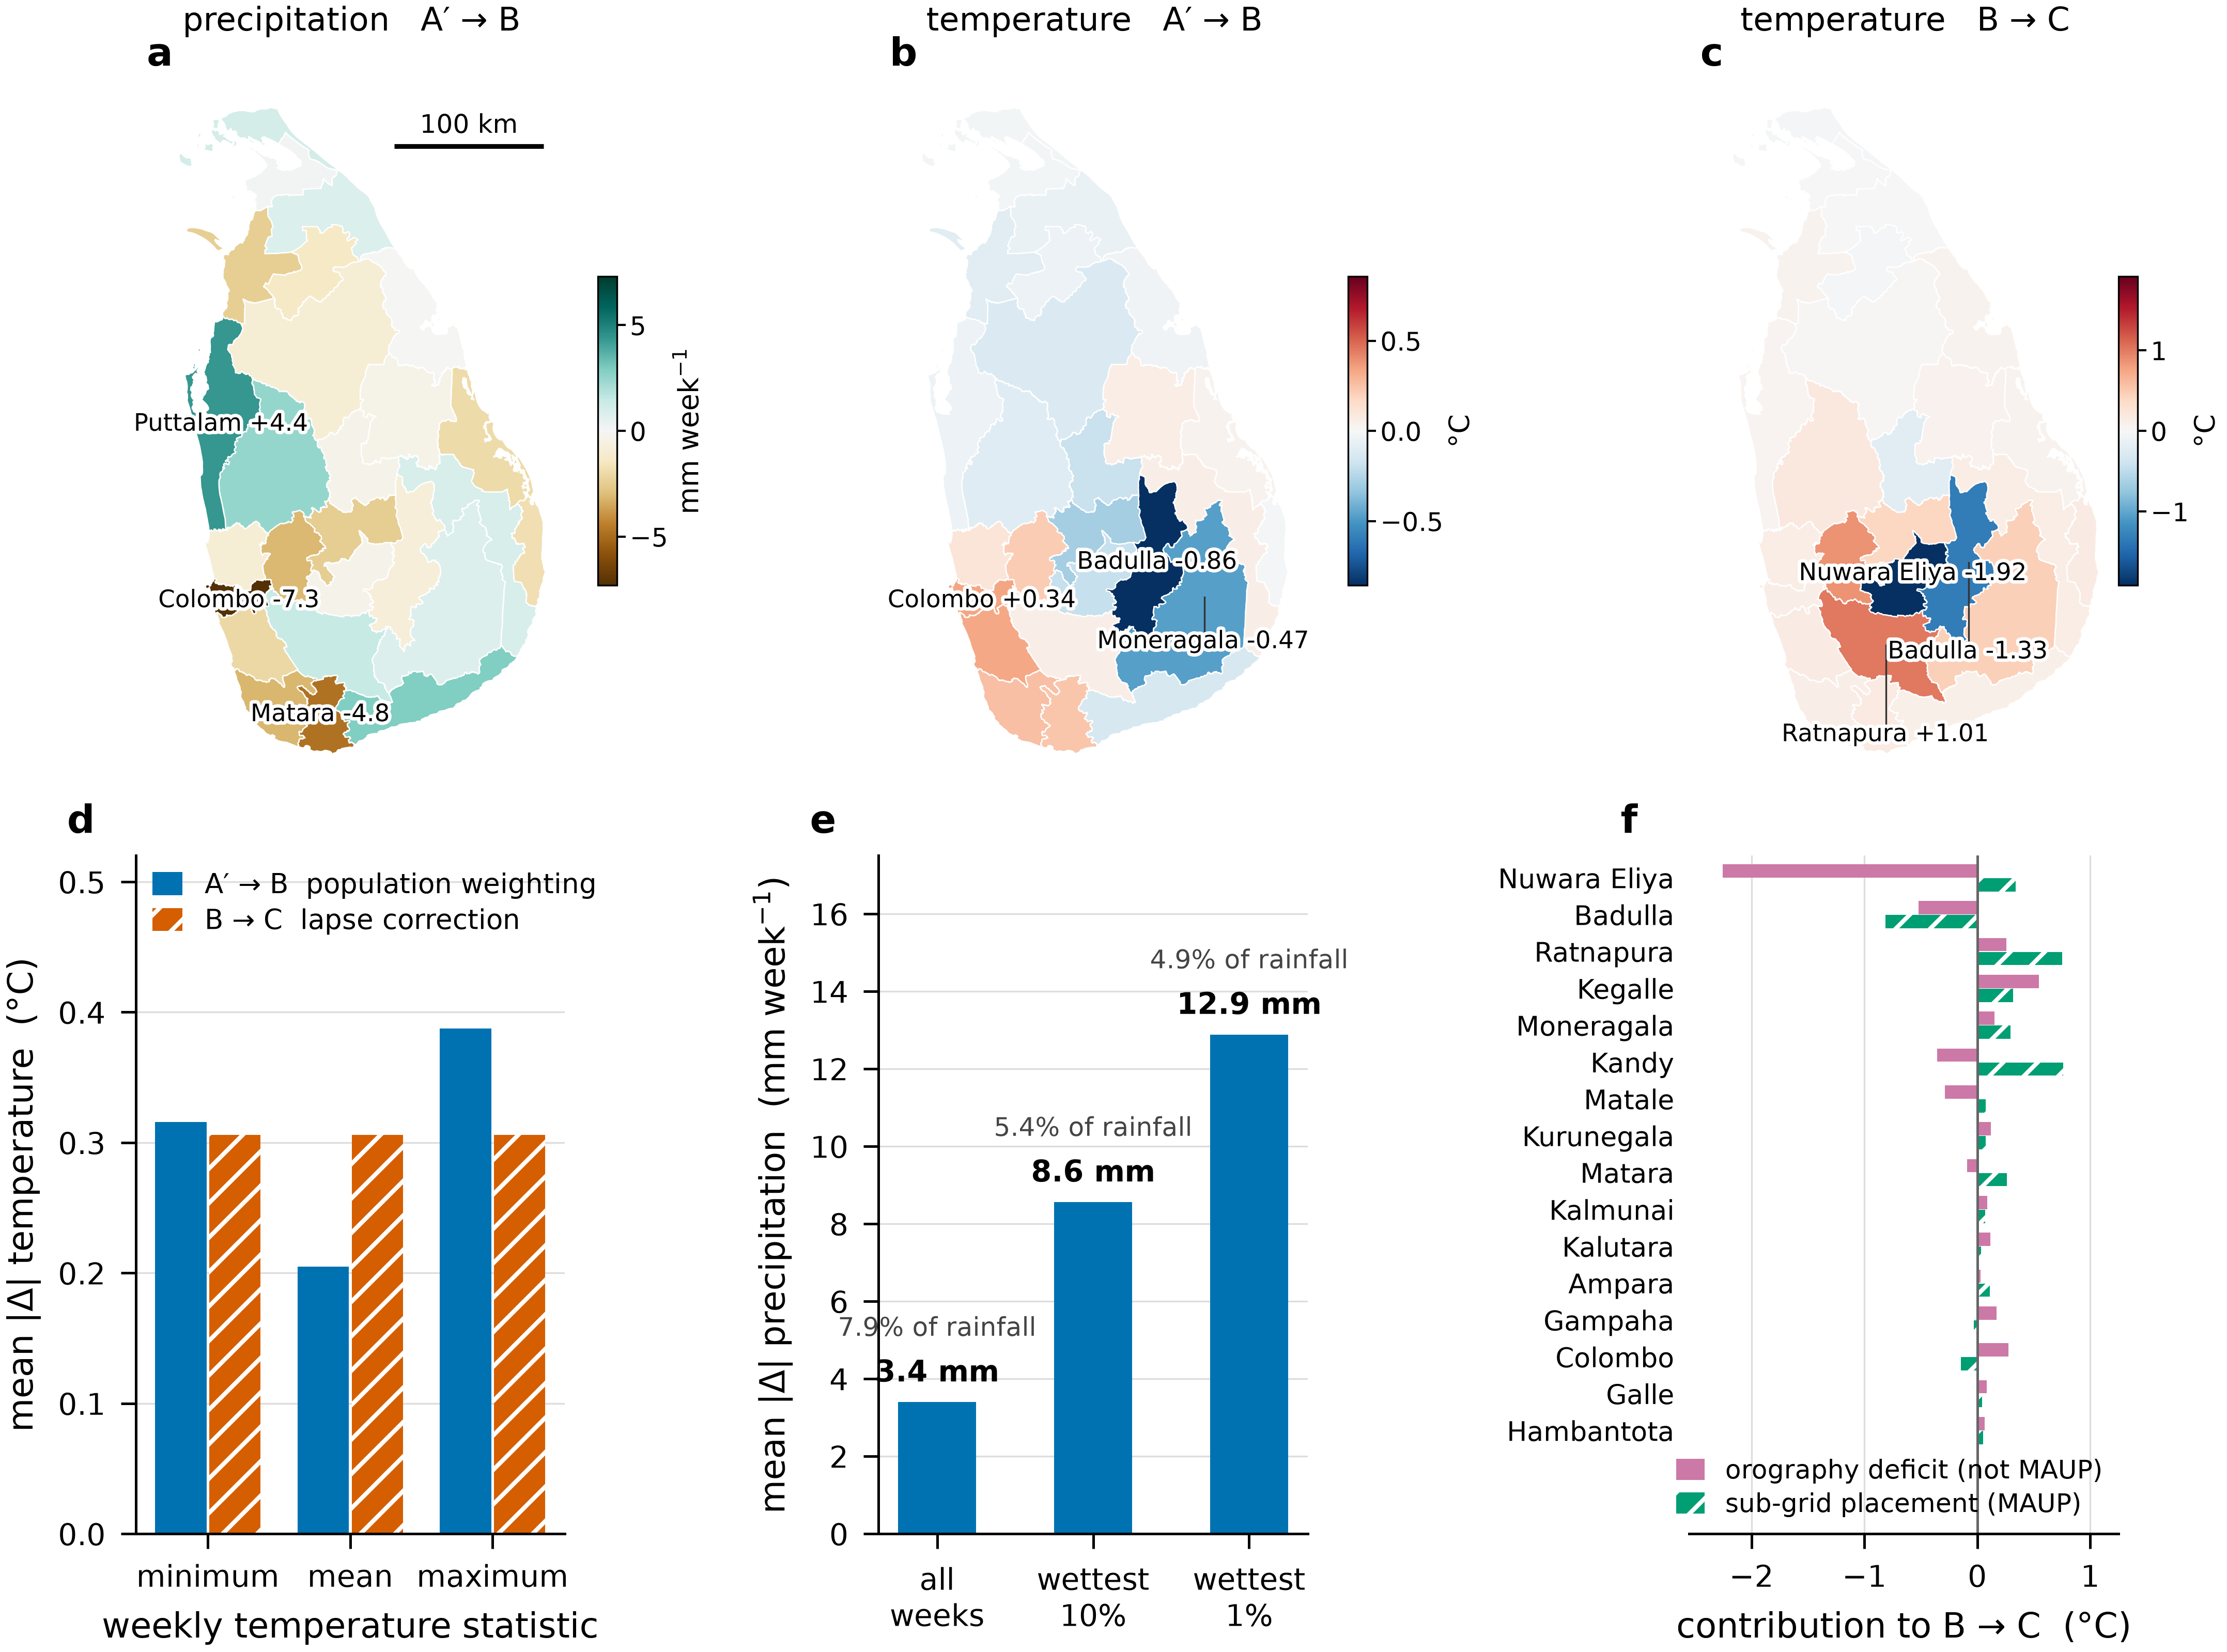
\includegraphics[width=\linewidth]{Manuscript_Figures/wp5/WP5_F2_exposure_contrast.pdf}
\caption{\textbf{Exposure construction contrast across the three-build ladder, Sri Lanka 2018--2025.}
Displacement in weekly district exposure attributable to the construction of the exposure variable alone, with the weather fields, geometry and temporal alignment held fixed. Panels show the per-district displacement for rainfall and temperature under population weighting (A$'\to$B) and under the additional lapse correction (B$\to$C), the decomposition of the mask step from the weighting step, the behaviour of the contrast in the wet tail where alerts fire, and the spatial pattern of each. Rainfall and temperature displacement are effectively uncorrelated across districts ($\rho=0.24$, $p=0.23$), so no single map identifies the exposure-sensitive districts. Maps are drawn in EPSG:32644. The three map panels use a diverging ramp that is symmetric in luminance and therefore does not survive greyscale reproduction; the largest movers are labelled numerically on the map face for that reason.}
\label{fig:wp5f2}
\end{figure}

\begin{figure}[htbp]
\centering
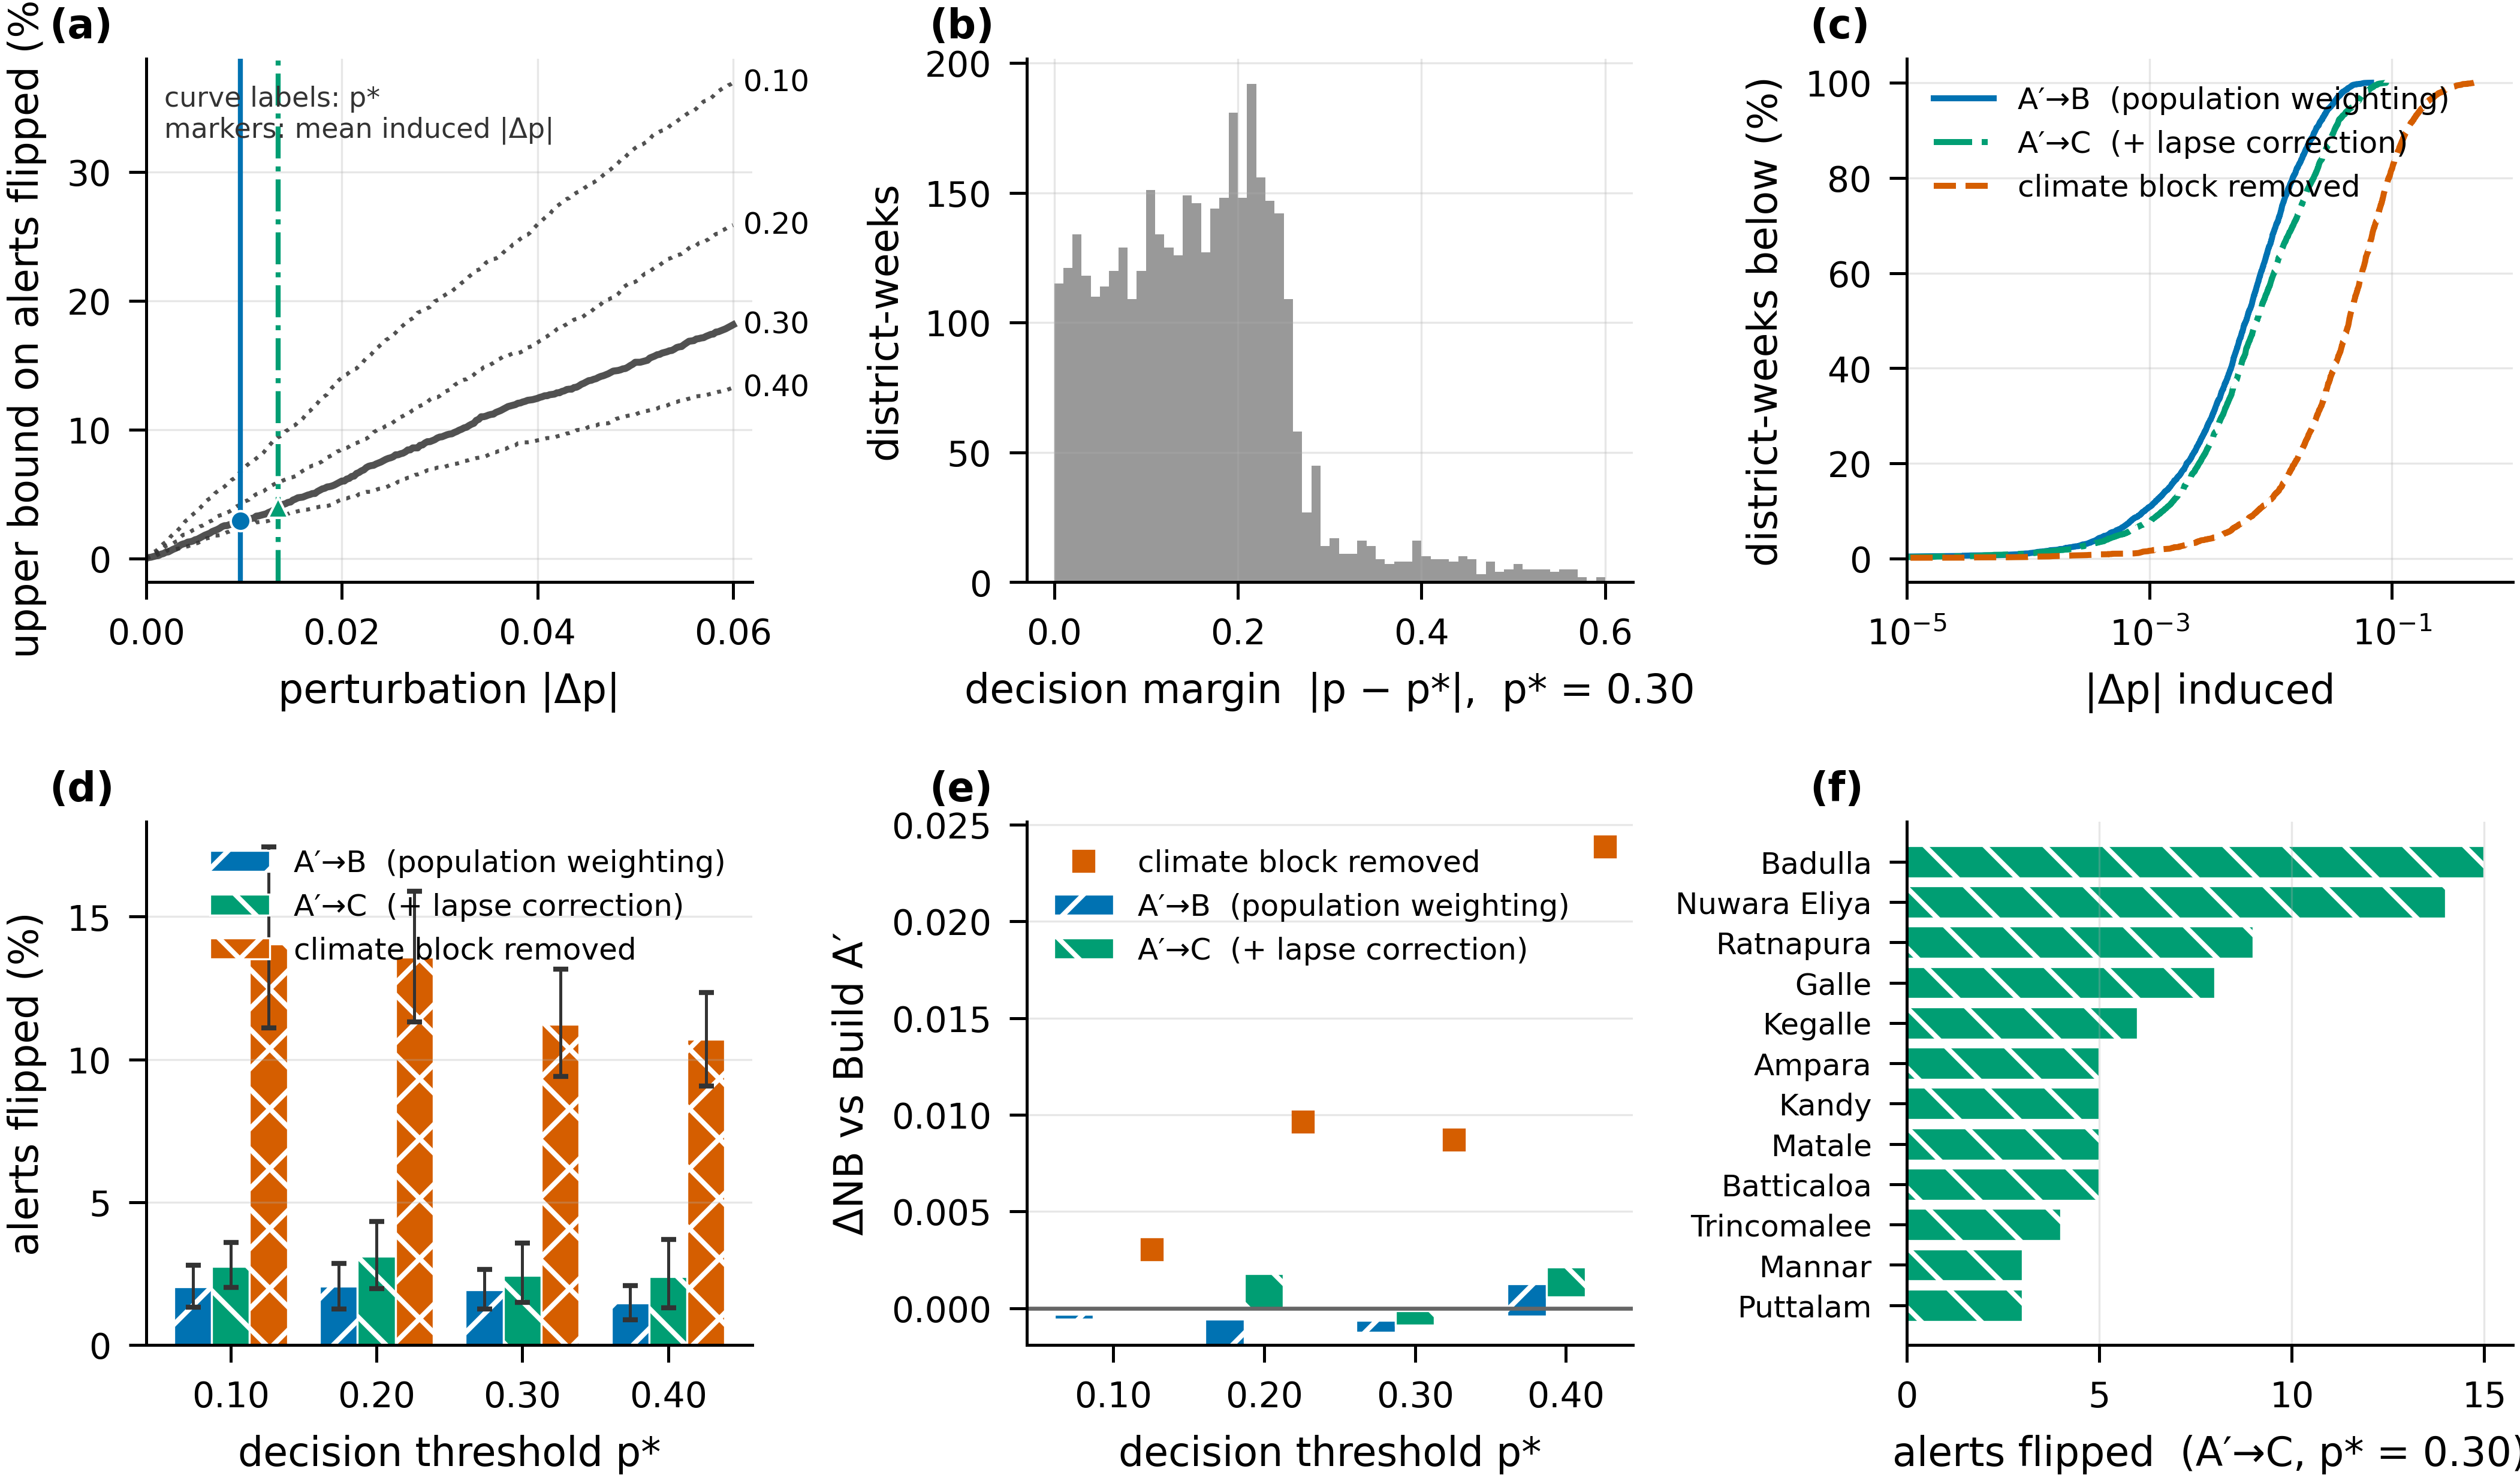
\includegraphics[width=\linewidth]{Manuscript_Figures/wp5/WP5_F7_decision_flip_envelope.pdf}
\caption{\textbf{Decision-flip envelope: exposure construction changes alerts that net benefit cannot see.}
Held-out panel of 3{,}926 district-weeks, 2023--2025. The exact flip curve gives the maximum share of alert decisions that any perturbation of a given size can change, as a property of the frozen predictions alone; estimated flip counts for each exposure rung are bounded by it, and the effect of deleting the entire climate block provides the observed ceiling. The lower panels show why the change in net benefit stays within $\pm0.0023$ while flip counts are clearly non-zero: rows that flip lie near the decision threshold, and rows near the threshold have an event rate near it, which is by definition the break-even rate at which a flip is worth approximately zero net benefit in either direction.}
\label{fig:wp5f7}
\end{figure}

\begin{figure}[htbp]
\centering
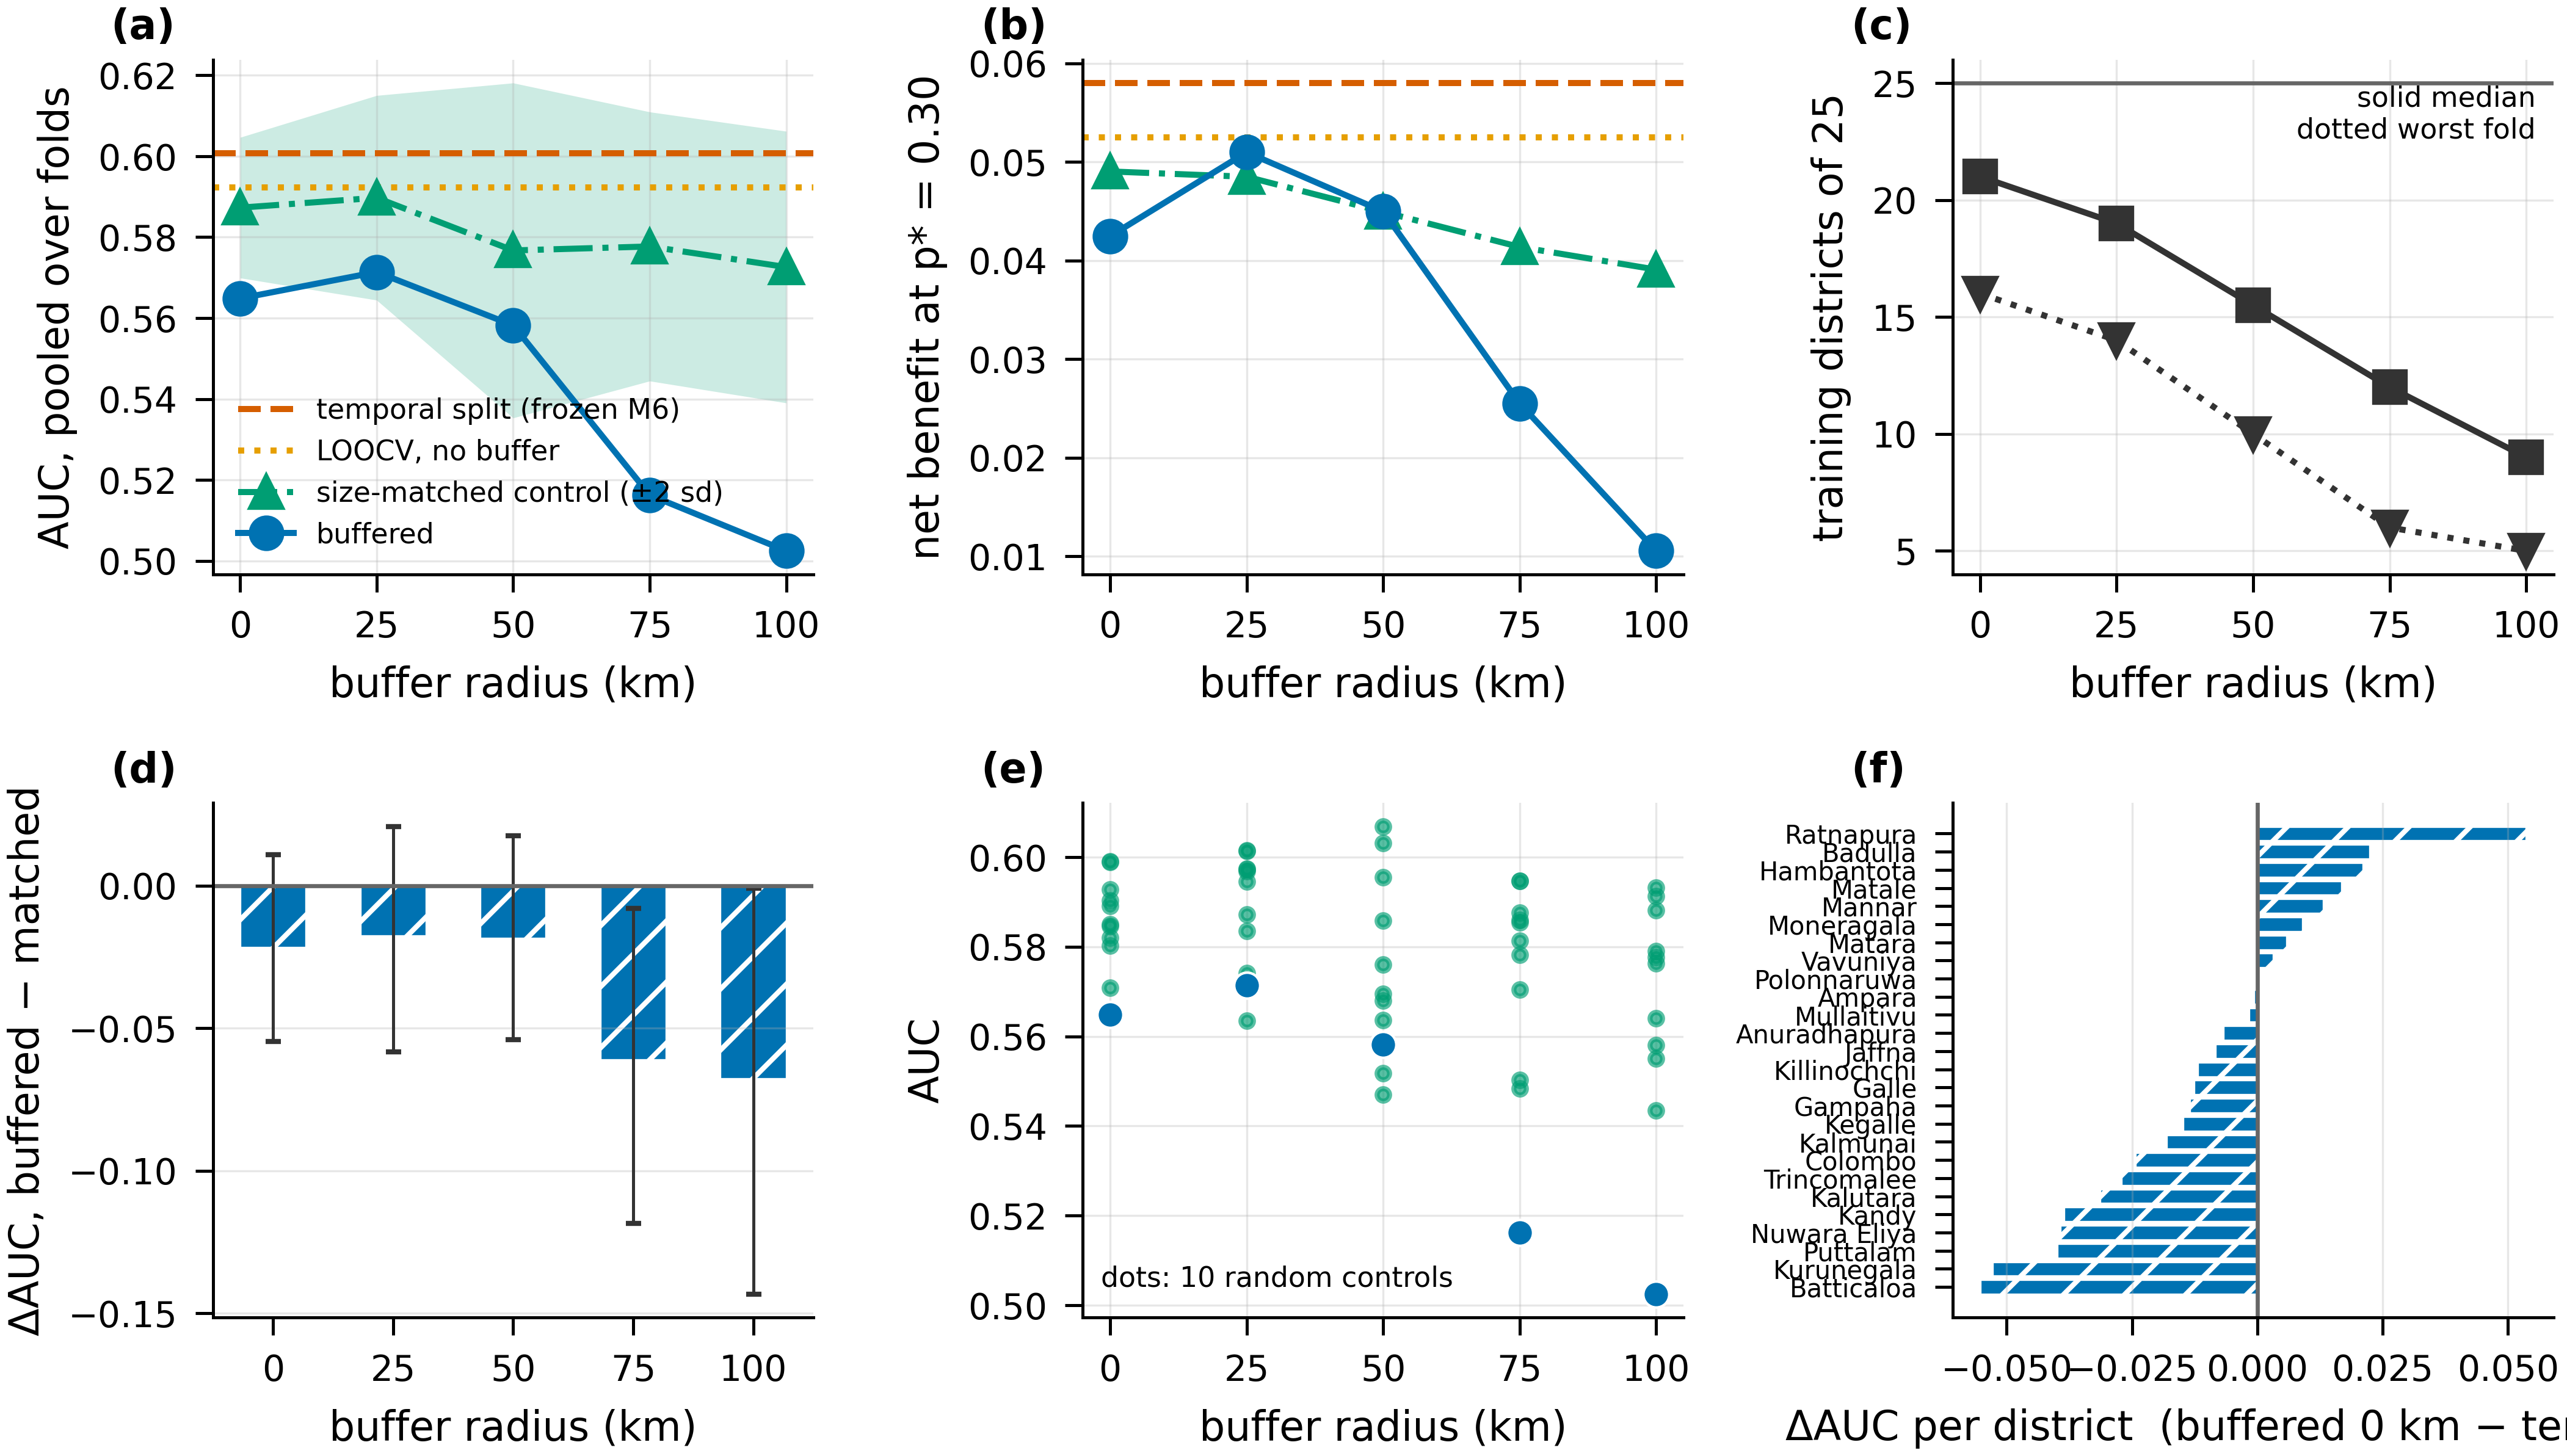
\includegraphics[width=\linewidth]{Manuscript_Figures/wp4/WP4_F_fold_effect_within_m6.pdf}
\caption{\textbf{What spatially buffered folds cost, measured against a size-matched control.}
Discrimination and calibration under buffered leave-one-out cross-validation at increasing buffer radius, each buffered fold matched to a random-district control trained on an identical number of districts so that the loss of training data is held fixed and the remaining gap is attributable to geography. Residual spatial autocorrelation is undetectable in these models at every distance band, yet performance still depends on having geographically proximate districts in training --- the two quantities disagree, so a residual-range analysis cannot be used to price the folds.}
\label{fig:wp4f}
\end{figure}

% =====================================================================
%  DISCUSSION MATERIAL (raw; not yet written to the Discussion's voice)
% =====================================================================
%
%  Four points from this work belong in the Discussion, in decreasing order of
%  reach beyond this study:
%
%  1. NET BENEFIT IS BLIND TO THRESHOLD-LOCAL PERTURBATIONS. This is a general
%     property of decision-curve analysis, not a WP5 result, and it qualifies
%     every sensitivity analysis in this literature that reads a small dNB as
%     "no decision effect" — including analyses reported elsewhere in this
%     paper. The recommendation is concrete: report a decision-flip count
%     alongside dNB whenever the perturbation acts near the threshold.
%
%  2. EXPOSURE CONSTRUCTION IS AN UNREPORTED ANALYST DEGREE OF FREEDOM that
%     carries 14–24% of the entire climate block's decision leverage. The
%     weighting choice matters ~4x more than the masking choice, and it is the
%     weighting that papers leave unstated.
%
%  3. RESIDUAL AUTOCORRELATION DOES NOT PRICE SPATIAL FOLDS. The conventional
%     design (choose the buffer from a residual range) fails here, in the
%     direction that matters: residuals look spatially clean while performance
%     depends materially on proximate training data.
%
%  4. THE COMPACT-COUNTRY CAVEAT. n=26 bounds what any of this can certify;
%     the Colombia block CV is where the well-powered spatial claim rests.
%
%  Deliberately NOT claimed anywhere above: that the published headline
%  comparison survives spatial CV (untestable without the design matrices);
%  that exposure construction changes dAUC or calibration (same); anything
%  about Colombia; any absolute performance figure for the geomatics-only model.
